The framework proposed by \citet{anmy11} represents the CMO problem as an integer programming problem.
When tested on a widely used benchmark, the Skolnick set \citep{gosk94}, the proposed algorithms for solving the optimization problem outperforms other existing exact algorithms both in terms of time efficiency and quality of bounds. To describe the formulation further, let us consider the contact maps of two proteins $P_1$ and $P_2$ given by $G_1 = (V_1,E_1)$ and $G_2 = (V_2,E_2)$, where $n_1$ is the number of vertices in $G_1$ and $n_2$ is the number of vertices in $G_2$. For convenience, contact maps of both the proteins will be represented by the index $m$ that takes value $1$ for $P_1$ and value $2$ for $P_2$. The right and left neighbour of any vertex $i$ in the $m^{\text{th}}$ protein is given by $\delta_m^+ = \{j | j>i ,(i,j) \in E_m)\}$ and  $\delta_m^- = \{j | j<i ,(j,i) \in E_m)\}$ respectively. For every edge $(i,j)\in E_1$ mapped to  $(k,l)\in E_2$, a non-crossing alignment happens when $i<j$ and $k<l$. Feasible alignments of two proteins $P_1$ and $P_2$ are given by non-crossing matchings in the complete bipartite graph $B$ with a vertex set $V_1\cup V_2$.
For every such non-crossing alignment, a weight $w_{ikjl}$ is introduced according to the following rule:
\begin{equation}
\label{rec11}
w_{ikjl}=\begin{cases}
    1, & \text{ if } (i,j) \in E_1 \text{ and } (k,l) \in E_2,\\
    0, & \text{ otherwise}.
  \end{cases}
\end{equation}
If $M$ represents the complete set of non-crossing matching in $B$, then $w(M)$ is the sum of all the weights over edges in $M$ and the CMO problem is nothing other than maximizing $w(M)$.

\begin{figure}[ht]
\centering
 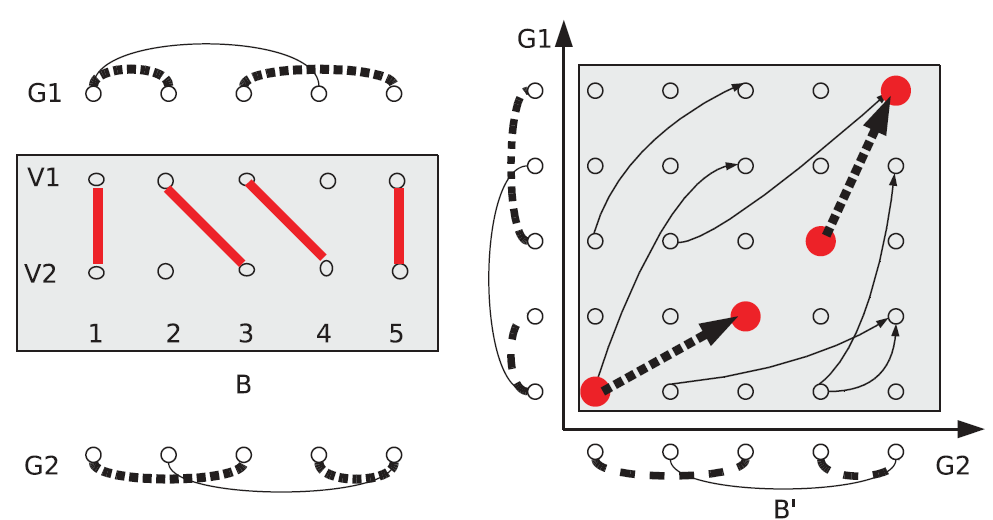
\includegraphics[width=0.7\textwidth]{pic1}
 \caption{Bipartite and Grid Graph Representation}
 \label{fig:Bipartite and Grid Graph Representation}
\end{figure}

Now, let us consider an interesting transformation of the problem also studied extensively in \citet{andonov04, andonov08}. The edges of $B$ are mapped onto a gird of size $n_1\times n_2$ which is denoted by $B^{\prime} = (V^{\prime},E^{\prime})$. The mapping abides by the following rule -- a vertex $(i,k) \in V^{\prime}$ if there exists an edge $(i,k)$ in $B$ and an arc $(i,k)(j,l) \in E^{\prime}$ if $w_{ikjl} = 1$. A bipartite graph $B$ and its corresponding grid graph transformation are illustrated in Fig. \ref{fig:Bipartite and Grid Graph Representation} \citep{anmy11}. In Fig. \ref{fig:Bipartite and Grid Graph Representation}, only the edges of the considered matching are shown. Further, let's consider ``feasible path" in this grid which is defined as an arbitrary sequence of vertices whose coordinates are arranged in increasing order. For example, in Fig. \ref{fig:Bipartite and Grid Graph Representation}, a feasible path is a path connecting the vertices $(1,1)$, $(2,3)$, $(3,4)$ and $(5,5)$.
Since, $M = \{(1,1)(2,3),(3,4)(5,5)\}$, according to the update rule given in Eq. \ref{rec11}, $w(M) =2$. One can 
see that the arcs $(1,1)(2,3)$ and $(3,4)(5,5)$ are activated only in Fig. \ref{fig:Bipartite and Grid Graph Representation} which contribute towards making $w(M)=2$. Therefore, in the transformed representation $B^{\prime}$, one can see that the objective is to maximize the number of such arcs whose vertex set forms the feasible path.

By assigning a binary variable $x_{ik}$ to each vertex $(i,k)\in B^\prime$ and a binary variable $y_{ikjl}$ to each arc $(i,k)(j,l)\in B^\prime$ and considering $X$ to be a feasible path in $B^\prime$, the maximum CMO problem can be represented as an integer programming problem as follows:
\begin{equation}
\label{rec1}
v(\mathbf{x},\mathbf{y}) = \max_{\mathbf{x},\mathbf{y}} \sum\limits_{(ik)(jl) \in E^{\prime}} y_{ikjl} \text{, subject to,}
\end{equation}
\begin{equation}
\label{rec2}
x_{ik}  \geq \sum\limits_{l \in \delta _2 ^+(k)}  y_{ikjl} ,	    j\in {\delta _1^+(i)}, i \in [1,n_1-1] , k \in [1,n_2-1],
\end{equation}
\begin{equation}
\label{rec3}
x_{ik}  \geq \sum\limits_{l \in \delta _2 ^-(k)}  y_{ikjl} ,	    j\in {\delta _1^-(i)}, i \in [2,n_1] , k \in [2,n_2],
\end{equation}
\begin{equation}
\label{rec4}
x_{ik}  \geq \sum\limits_{l \in \delta _1 ^+(i)}  y_{ikjl} ,	    l\in {\delta _2^+(k)}, i \in [1,n_1-1] , k \in [1,n_2-1],
\end{equation}
\begin{equation}
\label{rec5}
x_{ik}  \geq \sum\limits_{j \in \delta _2 ^-(i)}  y_{ikjl} ,	    l\in {\delta _2^-(k)}, i \in [2,n_1] , k \in [2,n_2],
\end{equation}
\begin{equation}
\label{rec6}
\{x_{ik}\} \in X,
\end{equation}
\begin{equation}
\label{rec7}
\sum\limits_{l=1}^k  x_{il} + \sum\limits_{j=1}^{i-1}  x_{jk} \leq 1  ,          i \in [1,n_1], k \in [1, n_2].
\end{equation}
Here, $\mathbf{x} = \{x_{ik}\}$ and $\mathbf{y} = \{y_{ikjl}\}$. A feasible path $X$ is constructed by taking a complete grid graph and then pruning the edges based on the constraints described above. To understand the first constraint (Eq. \ref{rec2}) in details, let us consider a CMO problem where the $i^{\text{th}}$ residue from one protein is mapped to the $k^{\text{th}}$ residue of the other protein. Considering that $(i,j)\in E_{1}$ and the fact that CMO is an order preserving bijection, $j$ can only be mapped to one point in the the second contact map \emph{i.e.}, $l$ in the second contact map will be unique. Constraint \ref{rec4} is similar to the constraint \ref{rec2} but corresponds to the reverse order. If there is an edge from $k$ to $i$ in the bipartite graph (\emph{i.e} $k^{\text{th}}$ residue from the second protein is mapped to $i^{\text{th}}$ residue in protein 1 )and if $(k,l)\in E_{2}$ is an edge in the second contact map, then $j$(the point $l$ can be mapped to) of the first contact map should also be unique. Here the summation signifies that for all values of $l$, only one can be 1,the remaining has to be 0. Similarly constraints \ref{rec4} and \ref{rec5} are constructed. The sets of the right and left neighbours are useful to formulate the same. Again weight $w_{ikjl}$ is one when the matching is non crossing, so the arc $(i,k)(j,l)$ is activated i.e. $y_{ikjl} = 1$ iff $x_{ik} = 1$ and $x_{jl} = 1$.

Constraint \ref{rec7} can be understood with the following example. Let $i$ be any residue in $P_1$. Now if $i$ is mapped to $k$ in $P_2$,then $x_{ik}$ is $1$ and it satisfies the constraint. If $i$ is not mapped to $k$, then either $i$ will be mapped to any element from $1$ to $(k-1)$ or $k$ will be mapped to any element from $1$ to $(i-1)$. This also reiterates the fact that there is only one bijective mapping between a residue in one protein to the other in another protein. Again, this mapping should be non-crossing, thereby reassuring order-preserving bijection.
